%!TEX root = ../my_thesis.tex
\chapter{Processeurs personnalisés à faible consommation pour le décodage SC} % (fold)
\label{chap:tensilica}

\vspace*{\fill}
\minitocTITI
\vspace*{\fill}
\newpage

\section*{Introduction}
Afin de tendre vers un réseau virtualisé de type Cloud-RAN, les implémentations logicielles des fonctions de traitement du signal dans les infrastructures de communication radio sont encouragées. Dans le chapitre précédent, de telles implémentations sont présentées pour les algorithmes de décodage polaire à liste. De hauts débits peuvent être atteints, et la flexibilité et la généricité de ces décodeurs sont très importantes. En utilisant des processeurs visant des systèmes électroniques embarqués, ces implémentations peuvent également gagner en efficacité énergétique.

Toutefois, les processeurs à usage général incluent de nombreuses unités matérielles destinées à exécuter efficacement de nombreuses et diverses applications. Mais toutes les unités matérielles ne sont pas utilisées dans la plupart des applications. Par exemple, dans les algorithmes de décodage de canal, toutes les unités de calcul à virgule flottante sont inutiles puisqu'une représentation des données internes en virgule fixe est privilégiée. Ces unités matérielles consomment alors de l'énergie inutilement. Le profilage d'un décodeur polaire montre que la majeure partie du temps d'exécution est passé à réaliser un ensemble restreint de fonctions élémentaires. De plus, une part significative des instructions exécutées correspond à des opérations de sauvegarde et de chargement de données dans les registres.

Ces observations poussent à envisager la conception d'un processeur programmable qui exclurait les unités matérielles inutiles des processeurs à usage général, tout en intégrant des unités de calculs spécialisées dans la réalisation efficace des fonctions élémentaires de décodage de codes polaires. Une telle architecture doit permettre de conserver une grande flexibilité nécessaire à la virtualisation des réseaux, tout en garantissant un niveau de performance se rapprochant des architectures dédiées. Ce type de processeurs entre dans la catégorie des processeurs à jeu d'instructions spécifique à l'application (ASIP: Application Specific Instruction-set Processor).

Les Chapitres \ref{chap:tensilica} et \ref{chap:tta} de ce manuscrit présentent deux architectures de processeurs ASIP spécialisées dans le décodage de code polaire. Ces deux architectures ont été conçues selon des méthodologies de conception différentes. La première méthodologie développée dans ce chapitre correspond à la spécialisation d'un processeur de base. Dans la section \ref{sec:asips}, le concept d'ASIP est introduit, et la méthodologie utilisée pour la première architecture est décrite. Dans la section \ref{sec:tensilica_design}, la conception de l'ASIP est détaillée. Enfin les résultats d'implémentation et les performances de l'architecture en termes de débit, latence, complexité matérielle et consommation énergétiques sont présentés et discutés dans la section \ref{sec:tensilica_res}.


\section{Les processeurs à jeu d'instructions spécifique à l'application}
\label{sec:asips}

Une des architectures ASIP que nous avons développées est basée sur un processeur de type RISC (Reduced Instruction Set Computer). Dans une première sous-section, les principes des architectures RISC sont présentés. Le concept d'ASIP est ensuite introduit. Les méthodologies de conceptions d'ASIP peuvent être divisée en deux groupes que nous détaillons. Le flot de conception de l'outil logiciel retenu pour concevoir ce premier ASIP sera ensuite présenté.

\subsection{Les processeurs RISC}
\label{subsec:risc}
\begin{figure}[t]
\centering
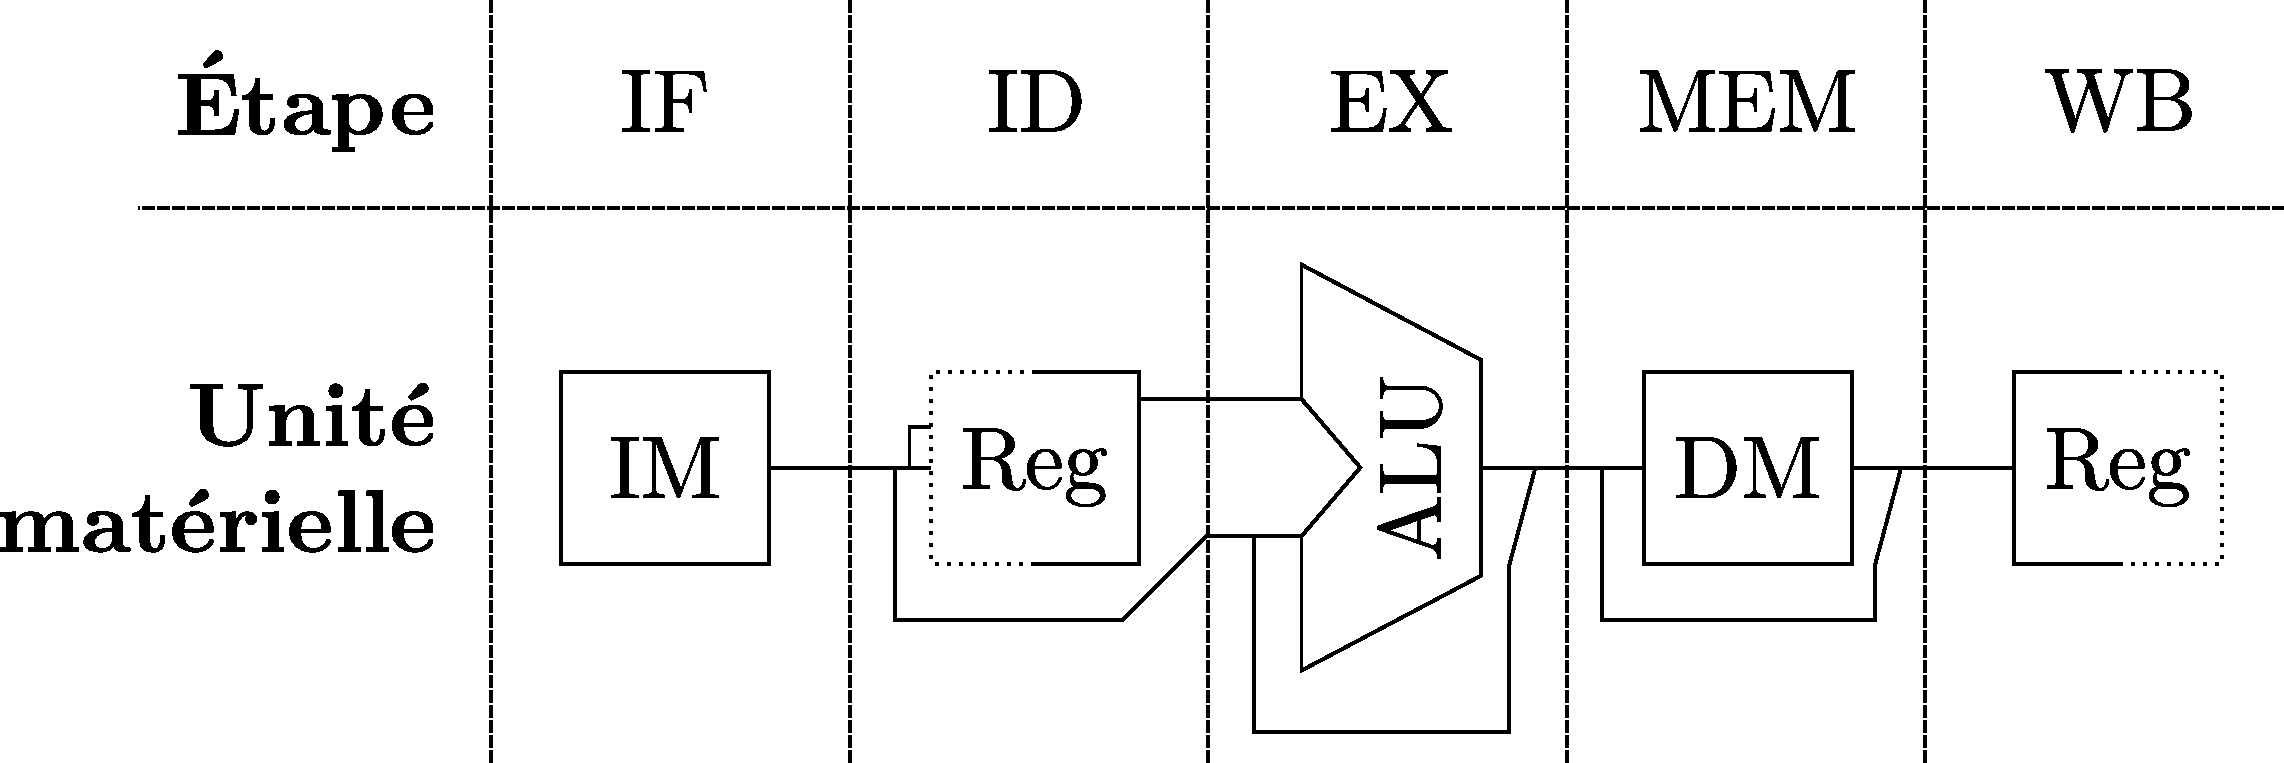
\includegraphics[width=\textwidth]{main/ch3_fig/stages}
\caption{\'Etages d'un processeur RISC}
\label{fig:risc}
\end{figure}

Dans le domaine de l'embarqué, les processeurs utilisés sont souvent de type RISC. Cette classe de processeurs a été introduite dans \cite{hennessy2011computer}. Par une analyse statistique et quantitative des applications traitées par les architectures de processeurs, les auteurs ont abouti à une microarchitecture de processeurs composée de 5 étages. Une unité matérielle est associée à chacun des étages, comme montré dans la Figure \ref{fig:risc}.

\begin{itemize}
  \item Le premier étage est l'étage de \textbf{chargement de l'instruction} (IF : Instruction Fetch) depuis la \textit{mémoire d'instruction} (IM : Instruction Memory). A chaque cycle d'horloge, une nouvelle instruction est chargée dans un registre spécialisé, nommé registre d'instruction. L'adresse en mémoire de l'instruction à charger est déterminée par le pointeur d'instruction, registre incrémenté automatiquement à chaque cycle d'horloge. L'instruction détermine l'opération qui à effectuer par le processeur dans les étages suivants. Il peut s'agir d'instructions arithmétiques et logiques, d'instructions de chargement et de sauvegarde depuis et vers la mémoire, ou bien d'instructions de branchement et de sauts. Ces dernières permettent de se déplacer dans la mémoire d'instructions. L'instruction contient également des informations sur les registres qui doivent être lus ou écrits, ainsi que des adresses mémoire dans le cas d'opérations de chargement ou de sauvegarde.

  \item Le deuxième étage correspond au \textbf{décodage de l'instruction} (ID : Instruction Decode) et à la lecture de la \textit{file de registres} (RF : Register File) spécifié(s) par l'instruction. Divers signaux de contrôle, qui seront utilisés dans les étages suivants, sont générés, selon l'instruction décodée.

  \item Le troisième étage est l'étage d'\textbf{exécution} (EX : Execution) dans lequel l'unité arithmétique et logique (ALU : Arithmetical and Logical Unit) effectue des opérations arithmétiques (+,-,*,/) et logiques (AND, OR, XOR,...). Ces opérations peuvent servir a effectuer des calculs d'adresses relatives ou à réaliser des opérations sur deux opérandes. Ces deux opérandes peuvent être deux registres ou bien un registre et une valeur immédiate intégrée dans l'instruction elle-même.

  \item Le quatrième étage est l'étage d'\textbf{accès à la mémoire}. S'il s'agit d'un chargement, une donnée est lue dans la \textit{mémoire de donnée} (DM : Data Memory) à l'adresse spécifiée dans un des registres. S'il s'agit d'une sauvegarde, la valeur d'un deuxième registre est écrite dans la DM.

  \item Le cinquième étage est l'étage d'\textbf{écriture différée} (WB : write-back). Cette étage permet d'écrire le résultat dans la file de registres, que ce soit le résultat d'une opération effectuée par l'ALU ou bien une donnée lue dans la DM.
\end{itemize}

\begin{figure}[t]
\centering
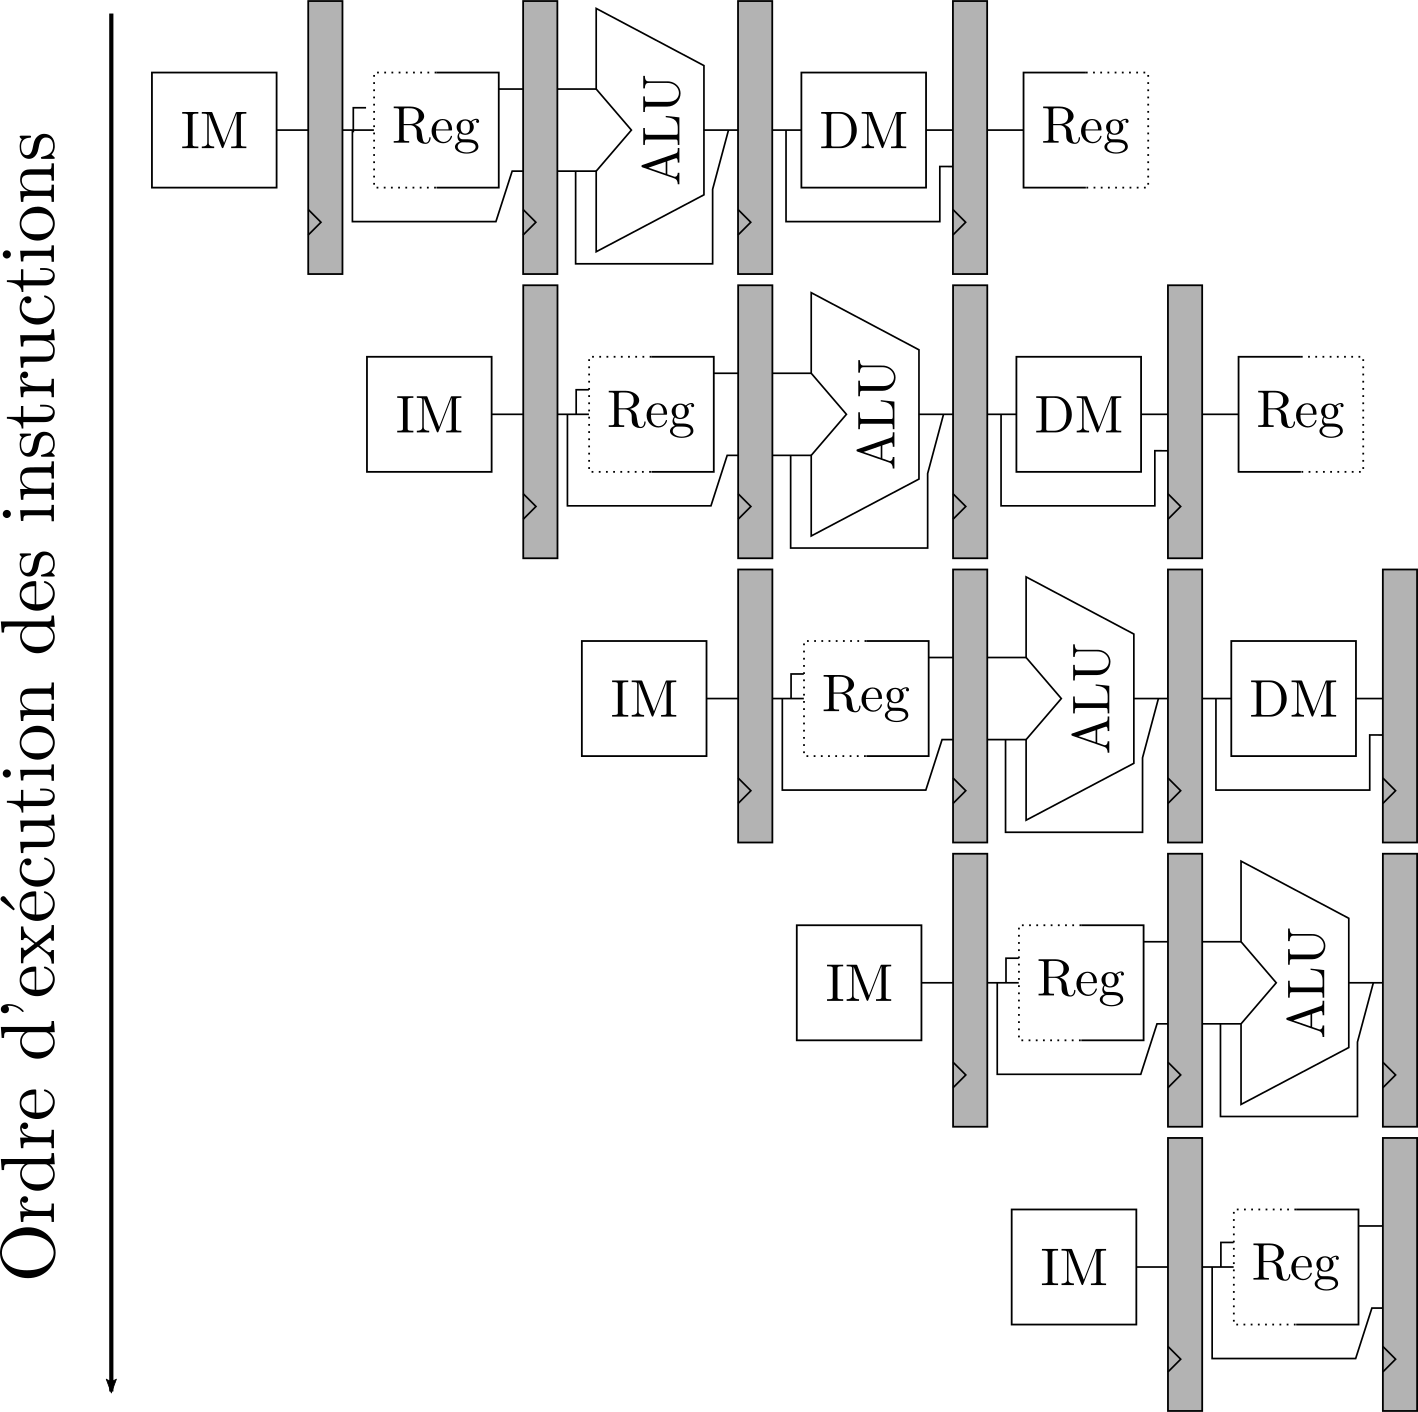
\includegraphics[width=0.75\textwidth]{main/ch3_fig/pipelines}
\caption{Structure et fonctionnement du pipeline RISC classique à 5 étages.}
\label{fig:pipelines}
\end{figure}


L'ajout de registres de pipeline comme illustré dans la Figure~\ref{fig:pipelines} permet d'isoler chacun des étages. Ainsi à chaque cycle d'horloge, une instruction est transmise d'un étage au suivant. Si une instruction est initiée à chaque cycle d'horloge, alors la performance du processeur sera 5 fois supérieure à celle d'un processeur sans registre de pipeline.

Nous venons d'introduire l'architecture RISC telle que définie dans \cite{hennessy2011computer}. Cette dernière fait figure de référence dans le domaine des architectures de processeur. En effet, cette organisation en pipeline à cinq étages, à quelques différences près, se retrouve actuellement dans de nombreux processeurs. L'architecture de base des processeurs XTensa proposés dans ce chapitre est une architecture de type RISC. Les processeurs XTensa sont une gamme de processeurs proposée par Tensilica, filiale de la société Cadence Design Systems.

\subsection{Les processeurs à jeu d'instructions spécifique à l'application}

Les méthodologies de conception des ASIP peuvent être divisées en deux famille. La première famille correspond à un flot de conception basé sur la spécification complète du processeur, représentée dans la Figure \ref{fig:methodo_adl}. Le modèle du processeur est décrit dans un langage de description architecturale (ADL : Architecture Description Language) \cite{mishra2011processor}. Ces langages de description permettent de définir précisément l'architecture d'un processeur. Ils peuvent être de différents types. Les ADLs structurels décrivent les composants des processeurs ainsi que leurs interconnexions. Les ADLs comportementaux décrivent quand à eux le comportement du jeu d'instructions du processeur. Des langages de description mixtes permettent quant à eux de décrire simultanément la structure et le comportement du processeur. Le flot de conception utilisé pour concevoir le processeur décrit dans le Chapitre \ref{chap:tta} utilise des ADLs comportementaux et structurels afin de générer le modèle matériel du processeur.


\begin{figure}[]
  \centering
  \subfloat[Flot basé sur la spécification complète du processeur.]{
  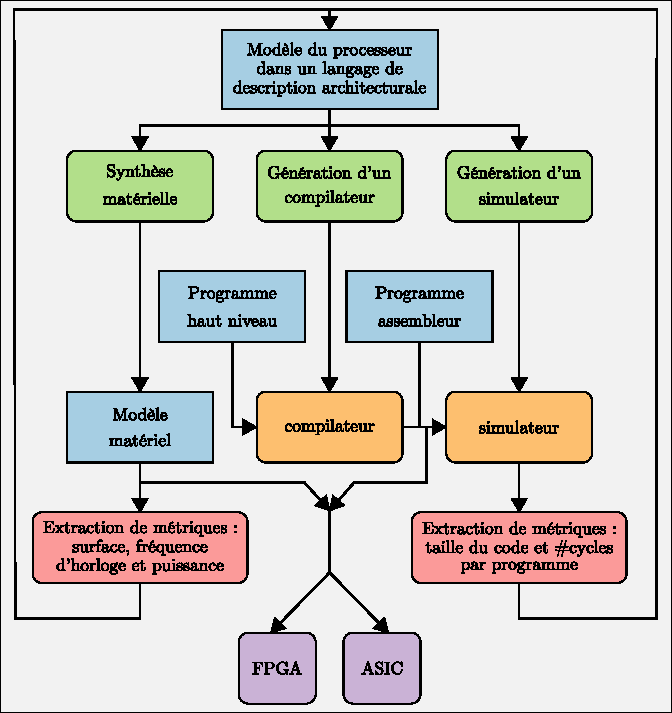
\includegraphics[scale=0.83]{main/ch3_fig/methodo_a}
  \label{fig:methodo_adl}
  }
  \\
  \subfloat[Flot basé sur la particularisation d’un processeur de base]{
  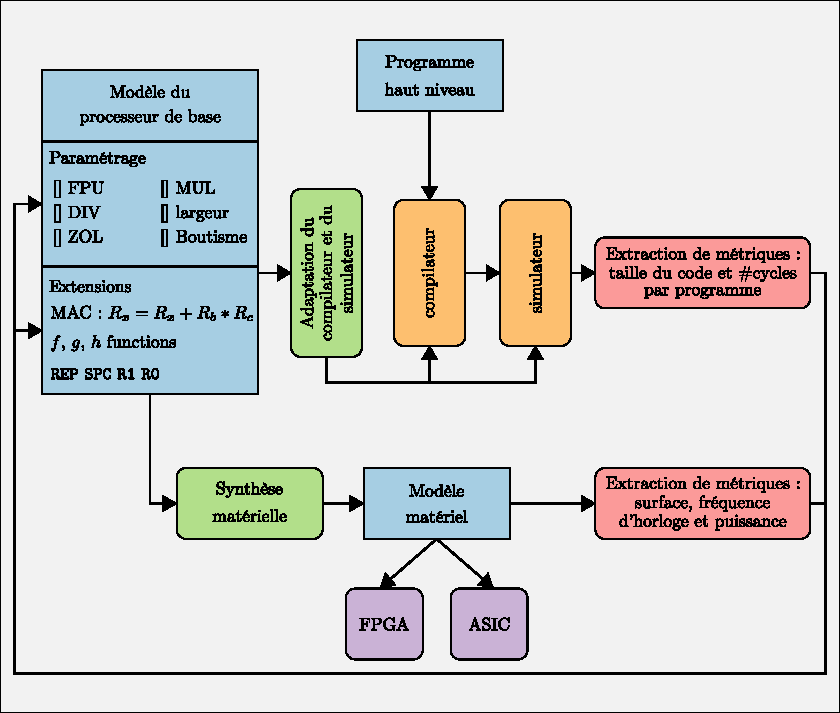
\includegraphics[scale=0.83]{main/ch3_fig/methodo_b}
  \label{fig:methodo_tensilica}
  }
  \caption{Méthodologies de conception des ASIP}
  \label{fig:asip_methods}
\end{figure}


La deuxième famille de méthodologies représentée dans la Figure \ref{fig:methodo_tensilica} correspond à l'approche utilisée par les outils de Tensilica pour concevoir l'ASIP proposé dans ce chapitre. Une architecture peu complexe en terme de surface occupée et à faible consommation constitue la brique de base du processeur. Dans le cas des outils de Tensilica, cette base est un processeur RISC doté d'un pipeline de 5 étages, tel que présenté dans la sous-section \ref{subsec:risc}. Afin de spécialiser le processeur, deux axes de conception sont disponibles. Premièrement, les principales unités matérielles du processeur RISC désignées dans la Figure \ref{fig:risc} sont paramétrables. Des caractéristiques telles que la profondeur et la largeur de la file de registre et / ou l'interface avec les mémoires sont modifiables. Comme indiqué sur la Figure \ref{fig:methodo_tensilica}, certaines fonctionnalités peuvent être ajoutées ou supprimées : unité de traitement reposant sur des représentations en virgule flottante (FPU : Floating Point Unit), unité d'accélération des multiplications (MUL) ou des divisions (DIV)... Le second axe est la possibilité d'étendre le jeu d'instructions. Grâce à un langage de description matérielle propre aux outils de Tensilica (TIE : Tensilica Instruction Extension) \cite{tie2017reference}, il est possible de spécialiser le processeur pour le décodage de codes polaires en ajoutant des unités matérielles dédiées aux fonctions élémentaires $f$, $g$et $h$.

Un des objectifs de la conception de processeurs par les méthodologies des conceptions que nous venons de présenter est de réduire le temps de conception des systèmes. Pour cela, des étapes clés dans la conception des processeurs sont automatisées. En effet, les suites logicielles de conception d'ASIPs permettent la génération automatique du compilateur, du simulateur, d'un outil de profilage et d'un outil de débogage. 

La génération du compilateur demeure critique. En effet, l'effort à déployer pour créer un compilateur associé à un processeur spécifique est considérable. En revanche, les compilateurs associés aux outils de conception d'ASIPs sont capables de s'adapter aux changements de structure du processeur. Ils proposent des optimisations spécifiques à la structure. Ils doivent également être capable de s'adapter au nombre de registres et les utiliser efficacement. Nous verrons dans le cas de notre processeur spécialisé dans le décodage de codes polaires que l'augmentation du nombre de registres à usage général favorise l'augmentation du débit de décodage. Le compilateur doit également être capable de gérer des modifications du pipeline et permettre un parallélisme d'instructions.

Le simulateur et l'outil de profilage générés permettent la validation fonctionnelle de l'architecture et du programme associé. Le nombre de cycles nécessaires à l'exécution du programme est obtenue à l'aide du simulateur. L'outil de profilage fournit des informations importantes sur la durée de l'exécution de sous-parties du programme afin de cibler les sections les plus consommatrices en temps. Ces métriques déterminent d'éventuelles modifications à apporter pour concevoir un nouveau modèle du processeur. L'outil de conceptions d'ASIP générera alors de nouveau un compilateur, un simulateur et un outil de profilage pour extraire les nouvelles métriques. Des itérations successives de ce flot permettent d'améliorer progressivement les performances recherchées de l'architecture et du programme considérés. Ce processus serait difficilement réalisable sans une telle suite d'outils automatisés.

Une fois l'architecture du processeur déterminée, le modèle matériel du processeur est généré. Ce modèle matériel peut être synthétisé et implémenté sur différentes cibles, ASIC ou FPGA. Il est alors possible d'extraire les métriques d'implémentations : fréquence de fonctionnement, surface occupée, puissance dissipée. De nouveau, des itérations sont possibles afin d'améliorer progressivement les performances.
Pour le processeur XTensa conçu dans le cadre de cette étude, la génération du modèle RTL n'a pas été possible par défaut de licence suffisante de l'outil de conception d'ASIPs. Seules des estimations de fréquence, de surface et de puissance dissipée sont fournies par l'outil. Cette absence de modèle matériel a été une des raisons pour lesquelles nous avons retenu par la suite d'autres méthodologies de conception telles que celle décrite dans le Chapitre \ref{chap:tta}.

\section{Un ASIP dédié au décodage de codes polaires}
\label{sec:tensilica_design}
\subsection{Paramétrage du processeur de base}
\subsubsection{Architecture de base}
La philosophie de conception de l'ASIP proposé est de réaliser l'ensemble des fonctions arithmétiques élémentaires pour le décodage de codes polaires à l'aide d'unités matérielles spécialisées. \`A l'inverse, les opérations de contrôle sont effectuées par l'architecture de référence du processeur XTensa. C'est la raison pour laquelle, l'architecture de référence a été simplifiée. Ainsi, les unités de calcul évoluées (unité de calcul en virgule flottante, MAC, ...) ont été supprimées.

\begin{figure}
\centering
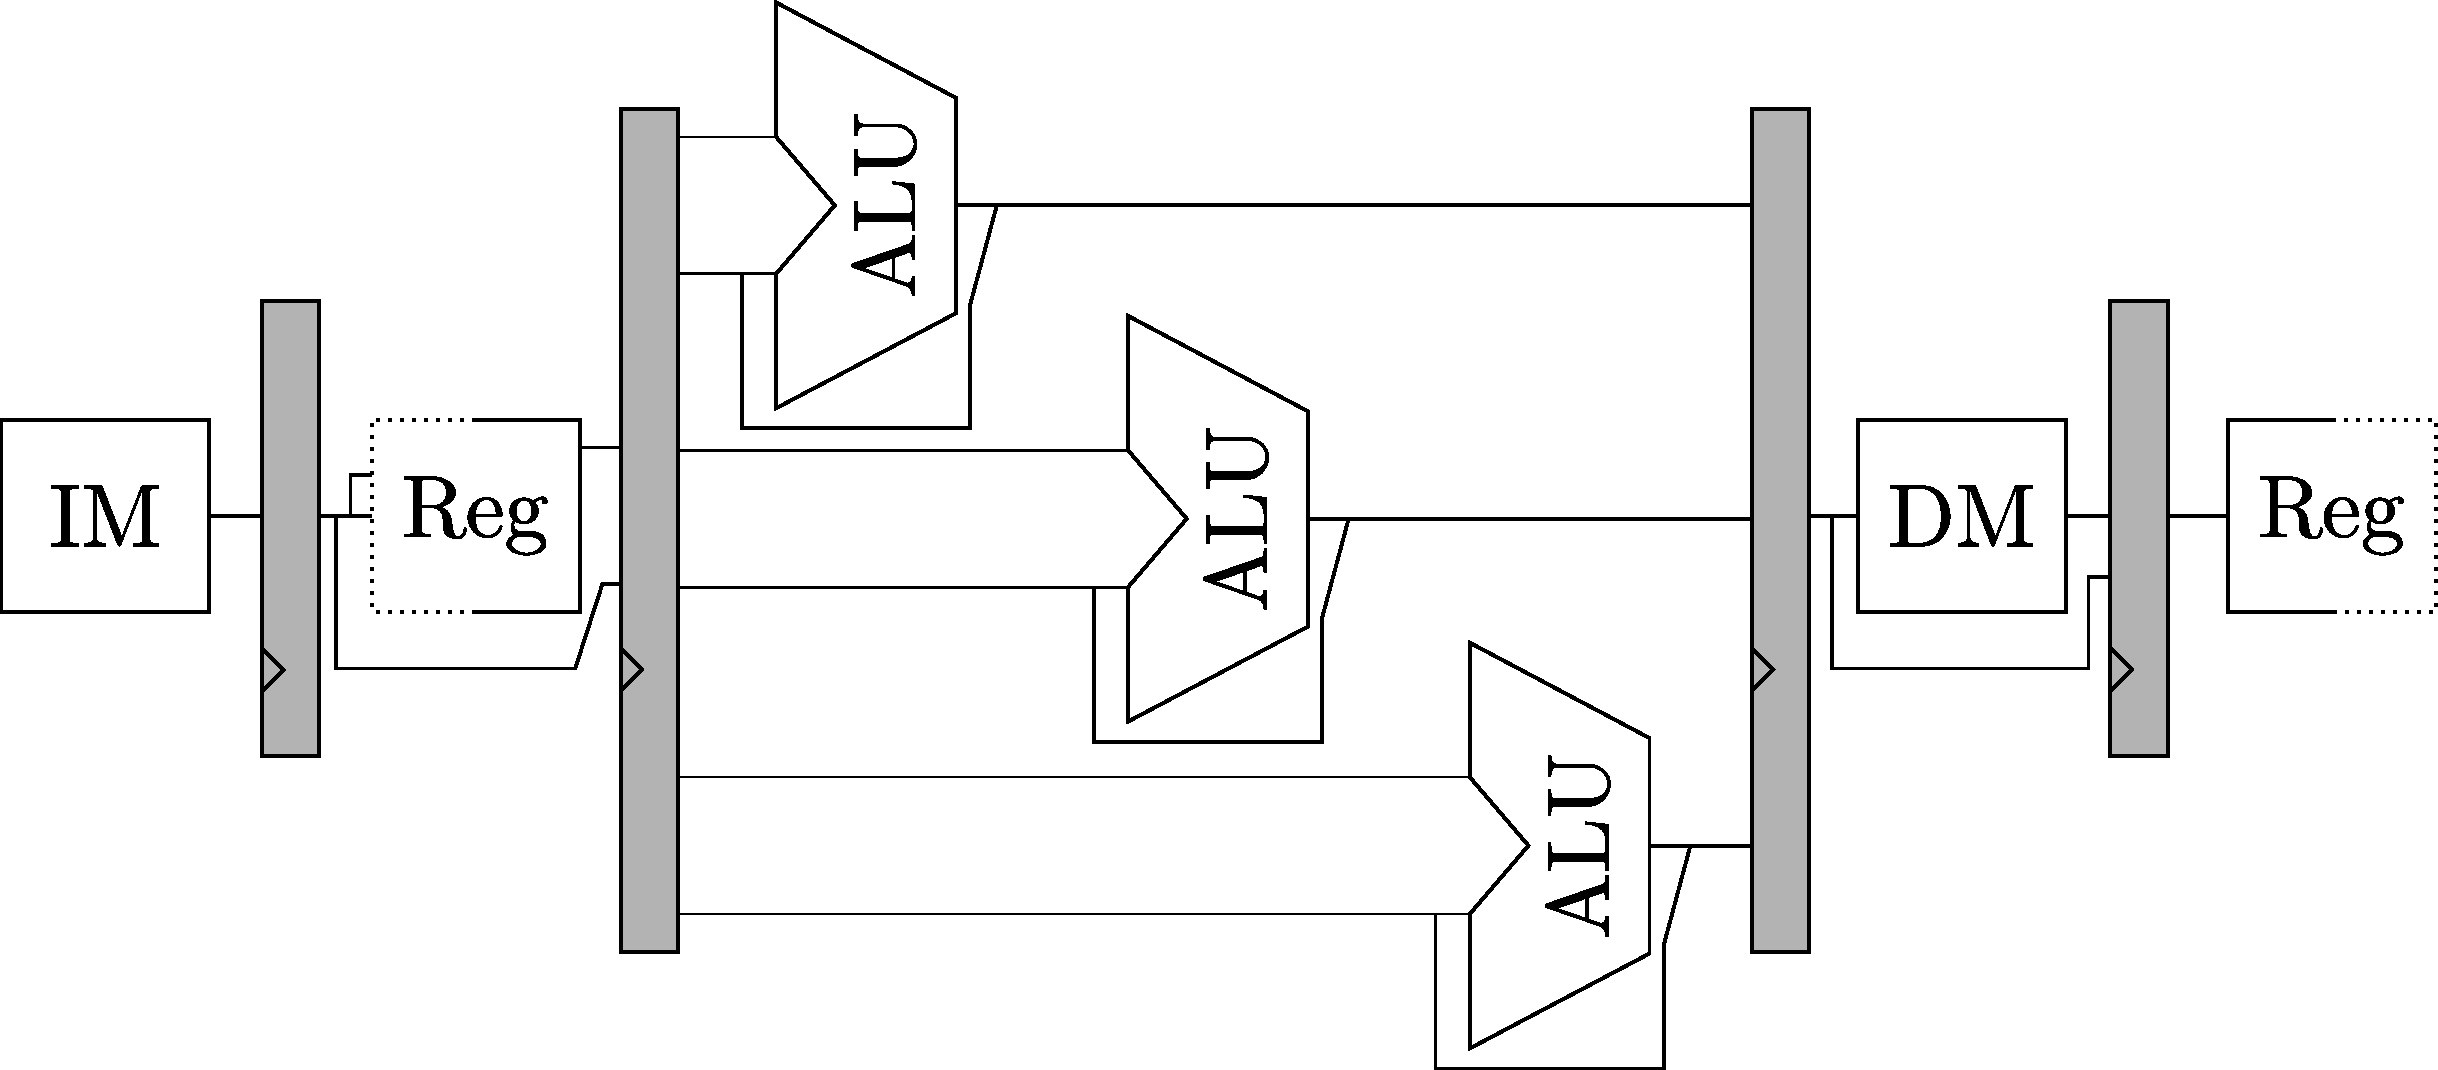
\includegraphics[width=\textwidth]{main/ch3_fig/flix}
\caption{Architecture associée à la fonctionnalité FLIX.}
\label{fig:flix}
\end{figure}

La fonctionnalité FLIX correspond à la possibilité d'ajouter des ALUs supplémentaires à la structure pipeline principale des processeurs XTensa. Cela permet au processeur d'exécuter plusieurs instructions en parallèle. Il est possible de configurer les instructions réalisées par chaque niveau pipeline. Notre choix s'est porté sur une configuration nommée FLIX3 prédéfinie par l'outil de conception. Ainsi, trois instructions faisant partie du jeu d'instruction de base peuvent être appliquées simultanément sur trois couples de données de 32 bits. Ce parallélisme d'instructions permet de réaliser plus rapidement les fonctions de contrôle et de calcul d'adresse. La fonctionnalité FLIX est détaillée dans la Figure \ref{fig:flix}.
La profondeur de la file de registres a été augmentée de 32 à 64 données de 32 bits. Cette modification permet une meilleure exploitation de l'augmentation du parallélisme d'instructions.

\subsubsection{Quantification des données}
Il est démontré dans \cite{sarkis_fast_2014} que des LLRs représentés sur 6 bits permettent d'atteindre les performances de décodage d'implémentations en virgule flottante. Cependant, il est plus simple dans une implémentation logicielle de représenter ces données sur 8 bits puisque les langages de programmation définissent de tels types de données. Comme montré dans \cite{leroux_hardware_2011}, $2^{n-d}$ LLRs doivent être stockés à un niveau $d$ de l'arbre de décodage. La taille de la mémoire permettant de stocker les LLRs est donc de $2^{n+1}-1$ octets.

Les sommes partielles sont des valeurs binaires. Cependant, encore une fois, la manipulation des sommes partielles dans le langage de description logicielle est plus aisée si un entier de 8 bits est utilisé pour représenter chaque somme partielle. Il serait cependant possible d'utiliser un entier pour représenter 8 sommes partielles, ce qui réduirait l'empreinte mémoire de celles-ci. Cependant cela nécessiterait cependant des opérations de masquage supplémentaires et cela introduit plus d'irrégularités au niveau des accès aux données.

\subsubsection{Configuration de la mémoire cache}
\begin{figure}
\centering
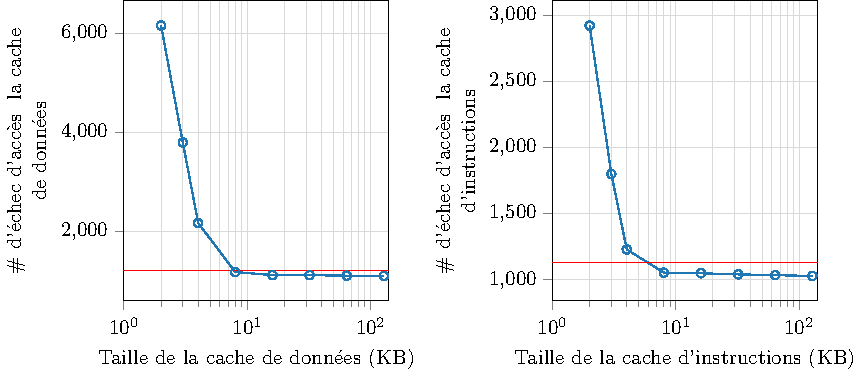
\includegraphics[width=\textwidth]{main/ch3_fig/curves/memory/tikz/memory}
\caption{Nombre d'échecs d'accès à la mémoire cache en fonction de la taille de la mémoire pour le décodage SC d'un code polaire de taille $N=1024$.}
\label{fig:tensilica_mem}
\end{figure}

Nous avons fait le choix d'augmenter au maximum le parallélisme des instructions élémentaires nécessaires au décodage de codes polaires. La taille maximum des registres du processeur XTensa, qui est donc la taille utilisée dans l'ASIP proposé, est de 512 bits. Afin de pouvoir charger et sauvegarder des données depuis et vers la mémoire cache en un seul cycle d'horloge, la largeur choisie pour une ligne de mémoire cache est également de 512 bits. La taille de ces mémoires ainsi que leur associativité est également configurable. Des expérimentations ont été réalisées afin de sélectionner ces valeurs. Dans tous les cas testés, un associativité à 4 voies pour les mémoires d'instructions et de données permet de meilleures performances.

Le scenario envisagé pour la conception du processeur est celui des canaux de contrôle du standard 5G tel que défini dans \cite{3gpp_ts_2017}. La taille du plus grand code polaire à décoder est $N=1024$. Les mémoires du processeur ont donc été dimensionnées en conséquence.
Bien que le plus petit nombre d'échec d'accès à la mémoire cache soit atteint pour la taille de cache la plus grande (128 Ko), une mémoire d'instruction de 8 Ko ainsi qu'une mémoire de données de 8 Ko sont suffisantes pour atteindre un nombre d'échecs de cache seulement 10 \% plus grand que la valeur optimale. Les mesures réalisées sont reportées dans la Figure \ref{fig:tensilica_mem}

\subsection{Ressources calculatoires utilisées dans les implémentations matérielles de l'état-de-l'art.}
\label{subsec:hard_sc}

\begin{figure}[t]
\centering
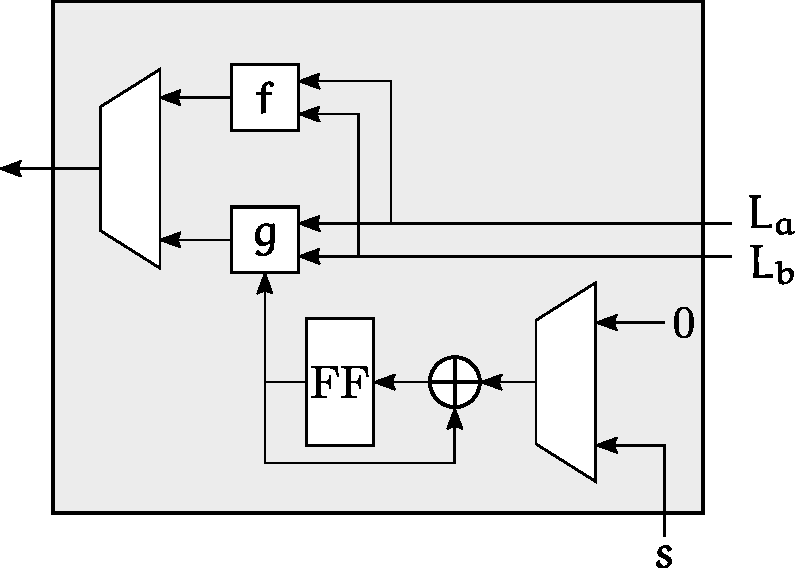
\includegraphics[scale=0.75]{main/ch3_fig/PE}
\caption{Unité matérielle élémentaire (PE : Processing Element).}
\label{fig:pe}
\end{figure}


Les instructions spécialisées choisies pour étendre le jeu d'instructions de l'ASIP s'inspirent des unités de traitement développées dans la littérature pour les circuits dédiés au décodage de codes polaires SC. Dans \cite{leroux_hardware_2011} plusieurs architectures furent proposées. La première architecture proposée est l'architecture \og papillon \fg. Lors du décodage, la fonction $f$ doit être appliqué $N/2$ fois à chaque niveau de l'arbre, et la fonction $g$ également. Au total, il est nécessaire d'appliquer $\frac{N}{2} \log N$ fois les fonctions $f$ et $g$. 

Pour cela, des unités matérielles élémentaires (PE : Processing Elements) sont utilisées.
Un PE permet de réaliser un calcul de $f$ et un calcul de $g$. Un tel élément est représenté dans la Figure \ref{fig:pe}.
Dans l'architecture \og papillon \fg, un PE est associé à chaque application des fonctions $f$ et $g$.
Il y a donc au total $\frac{N}{2} \log N$ PEs.
L'application de l'ensemble des fonctions $f$ ou des fonctions $g$ d'un \noeud de l'arbre est alors effectué en un cycle d'exécution.

Cependant, cette architecture est sous-optimale en termes de complexité.
L'ordonnancement de l'algorithme de décodage SC possède les propriétés suivantes :
\begin{itemize}
  \item Le nombre maximum de fonctions polaires élémentaires réalisées simultanément sur un \noeud est $\frac{N}{2}$,
  \item deux \noeuds successifs ne peuvent pas être traités simultanément.
\end{itemize}
En conséquence, les ressources de calculs alloués au traitement d'un \noeud de l'arbre peuvent être utilisé pour le traitements des \noeuds suivants.
Le niveau de parallélisme le plus élevé est $\frac{N}{2}$, donc $\frac{N}{2}$ PEs suffisent pour décoder l'ensemble de l'arbre sans modifier la latence de décodage.
Dans l'architecture \og ligne \fg, $\frac{N}{2}$ PEs sont donc partagées pour le traitement de tous les \noeuds de l'arbre. Sa latence est la même que celle de l'architecture \og papillon \fg.

Dans \cite{leroux_semi-parallel_2013} il est proposé de réduire le nombre de PEs grâce à l'introduction d'une architecture semi-parallèle, de manière similaires à des implémentations précédentes de décodeurs LDPC \cite{1049697}. Dans le décodeur \og ligne \fg, les N / 2 PEs ne sont tous utilisés simultanément que deux fois par mot de code décodé. Cela signifie que le taux d'utilisation des PEs est très faible. Il est donc possible de réduire le nombre de PEs sans impacter significativement le débit.
Cette réduction modifie légèrement l'ordonnancement l'algorithme. En effet les \noeuds nécessitant un nombre d'exécutions de fonctions polaires supérieures à $P$ nécessiteront plus d'un cycle d'horloge à décoder. Le rapport du nombre de PEs d'une architecture semi-parallèle sur le nombre de PEs d'une architecture \og ligne \fg est $N/2P$. Par exemple, pour $N=1024$ et $P=64$, le nombre de PEs est réduit d'un facteur $16$, tandis que le débit est réduit de $2\%$. Pour $N=2^{20}$ et $P=64$, le nombre de PEs est réduit d'un facteur $8192$, et le débit est réduit de moins de $10\%$. L'architecture semi-parallèle s'avère donc très pertinente.

L'architecture proposée dans \cite{sarkis_fast_2014} reprend le principe de l'architecture semi-parallèle. Cependant, les PEs sont modifiés pour intégrer des unités matérielles de traitement des \noeuds spécialisés \texttt{R1}, \texttt{SPC} et \texttt{REP}. Les PEs contiennent également une unité particulière \texttt{REP-SPC} permettant d’accélérer le traitement de deux \noeuds \texttt{REP} et \texttt{SPC} voisins. Ce motif particulier apparaît régulièrement pour le code polaire (32768,29492) considéré. Les unités \texttt{REP-SPC} ne sont pas utilisées dans le processeur proposé car elles n'apportent pas de gain significatif pour les tailles de codes traitées par le processeur que nous proposons ($N<1024$). 

Le dernier type de calcul nécessaire dans l'algorithme de décodage SC est le calcul des sommes partielles (fonction $h$). Dans les implémentations dédiées, les sommes partielles sont sockées dans des registres. Un réseau de portes \textit{ou-exclusif} routées sur ces registres permettent leurs mise à jours instantanées à chaque traitement d'une feuille de l'arbre de décodage. Ce réseau ne fait pas partie des PEs. Dans l'ASIP proposé, les sommes partielles sont stockées dans la mémoire de données, comme les LLRs, afin de les rendre accessibles par le processeur comme toute autre variable. La fonction $h$ fait donc partie des instructions spécialisées conçues pour étendre le jeu d'instructions de l'ASIP proposé.



% Les latences et le nombre de PEs nécessaire pour chaque architecture sont présentées dans le tableau \ref{tab:archis_sc}.

 % \begin{table}[h]
 %    \renewcommand{\arraystretch}{1.1}
 %    \centering
 %    \caption{Latence et nombre de PEs des trois architectures SC.}
 %    \label{tab:archis_sc}
 %    {\small\resizebox{\linewidth}{!}{
 %    \begin{tabular}{l | c  c }
 %    \textbf{Architecture}  & \textbf{Nombre de PEs} & \textbf{Latence (\# cycles)} \\
 %    \cmidrule(lr){1-1}
 %    \cmidrule(lr){2-2}
 %    \cmidrule(lr){3-3}
 %    \og papillon \fg       & $\frac{N}{2} \log N$   & $2N-2$
 %    \og ligne \fg          & $N/2$                  & $2N-2$
 %    \og semi-parallèle \fg & $P$                    & $2N + 
 %    \end{tabular}
 %    }}
 %  \end{table}


\subsection{Instructions spécialisées \textit{multi-registres}}
\label{subsec:multi_reg}

\begin{figure}
\centering
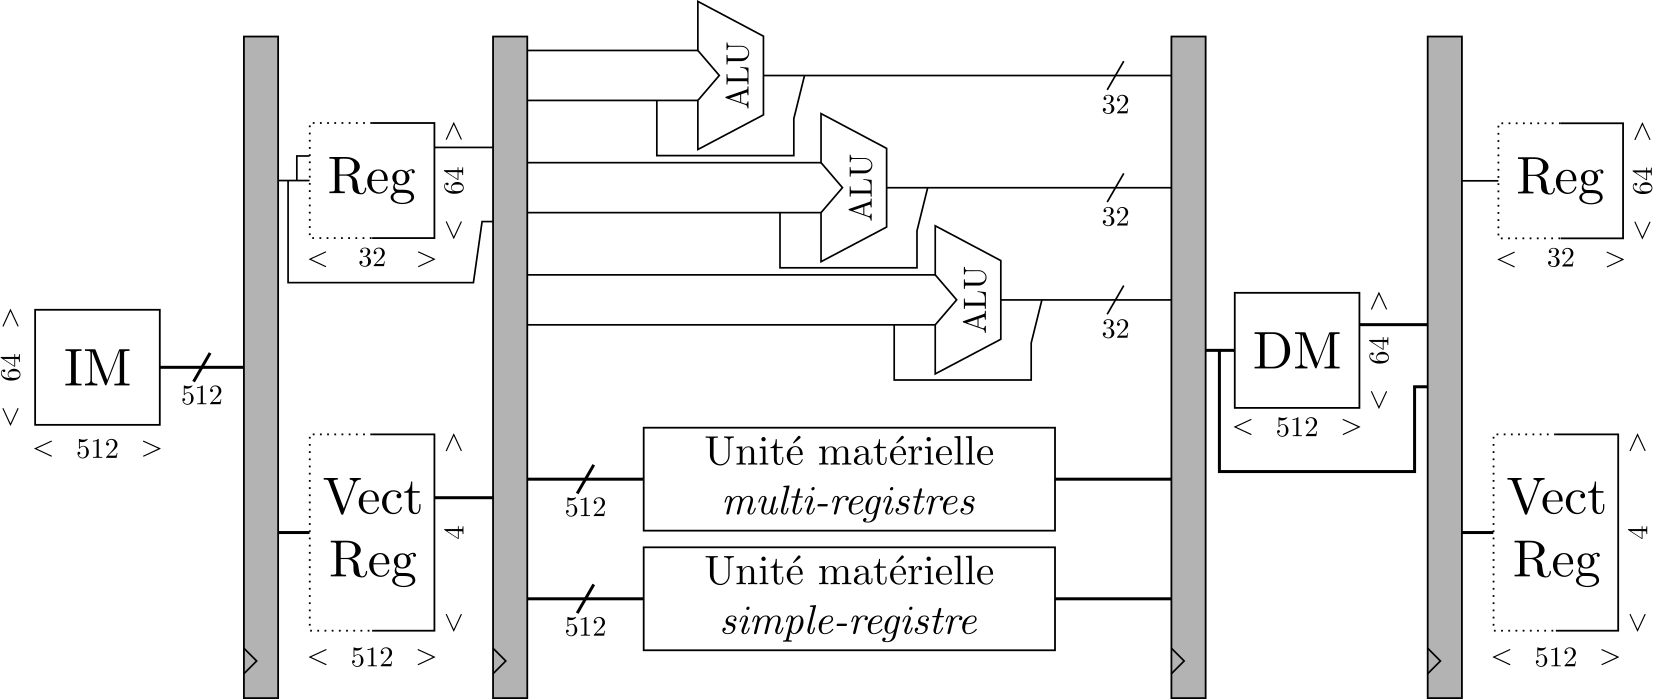
\includegraphics[width=\textwidth]{main/ch3_fig/full_tensilica}
\caption{Architecture de l'ASIP proposé.}
\label{fig:full_tensilica}
\end{figure}

Les instructions spécialisées réalisent des fonctions équivalentes à celles des PEs des architectures matérielles qui ont été présentées dans la sous-section \ref{subsec:hard_sc}. Il s'agit des fonctions $f$, $g$, \texttt{R1}, \texttt{R0}, \texttt{REP} et \texttt{SPC}. Deux types d'instructions spécialisées ont été conçues et ajoutées au processeur proposé comme montré dans \ref{fig:full_tensilica}. Les premières sont les instructions \textit{multi-registres} et les secondes les instructions \textit{simple-registre}. \'A l'image des PEs de l'architecture semi-parallèle, leur niveau parallélisme est fixé ($P=64$). Une file de registres vectoriel permet de stocker des données de 512 bits. Les instructions \textit{multi-registres} lisent et écrivent dans cette file de registres vectoriel.

Ces instructions spécialisées sont décrites à l'aide du langage TIE des outils de Tensilica.
L'implémentation de la fonction $f$ est représentée dans la Figure~\ref{fig:f_tie}. Les deux entrées sont les LLRs notés $L_a$ et $L_b$ et la sortie est notée $f(L_a,L_b)$. Ces deux entrées et la sortie correspondent à des registres de la file de registres vectoriels. Pour rendre claire l'illustration, le niveau de parallélisme dans la Figure~\ref{fig:f_tie} a été réduit à $P=4$. Dans la plupart des décodeurs polaires, pour réduire le chemin critique, les LLRs sont représentés au format \og signe-amplitude \fg : un bit est utilisé pour le signe, et le reste pour la valeur absolue, toujours positive. Dans notre implémentation, les valeurs négatives sont représentées en complément à deux, car il s'agit du mode de représentation utilisé dans les processeurs XTensa.
La fonction $g$ est représentée dans la Figure~\ref{fig:g_tie}. Elle consiste en une addition simple avec une inversion de signe selon la valeur de la somme partielle $s_a$.
La fonction $h$ n'est pas représentée, il s'agit simplement d'un \textit{ou-exclusif} entre les sommes partielles d'entrées. Les fonctions \texttt{R0} et \texttt{R1} sont également très simples, puisqu'il s'agit d'une mise à zéro dans le premier cas et d'un seuillage dans le deuxième. Le seuillage est une simple copie du bit de poids fort.
\begin{figure}[t]
  \centering
  \subfloat[Fonction $f$]{
  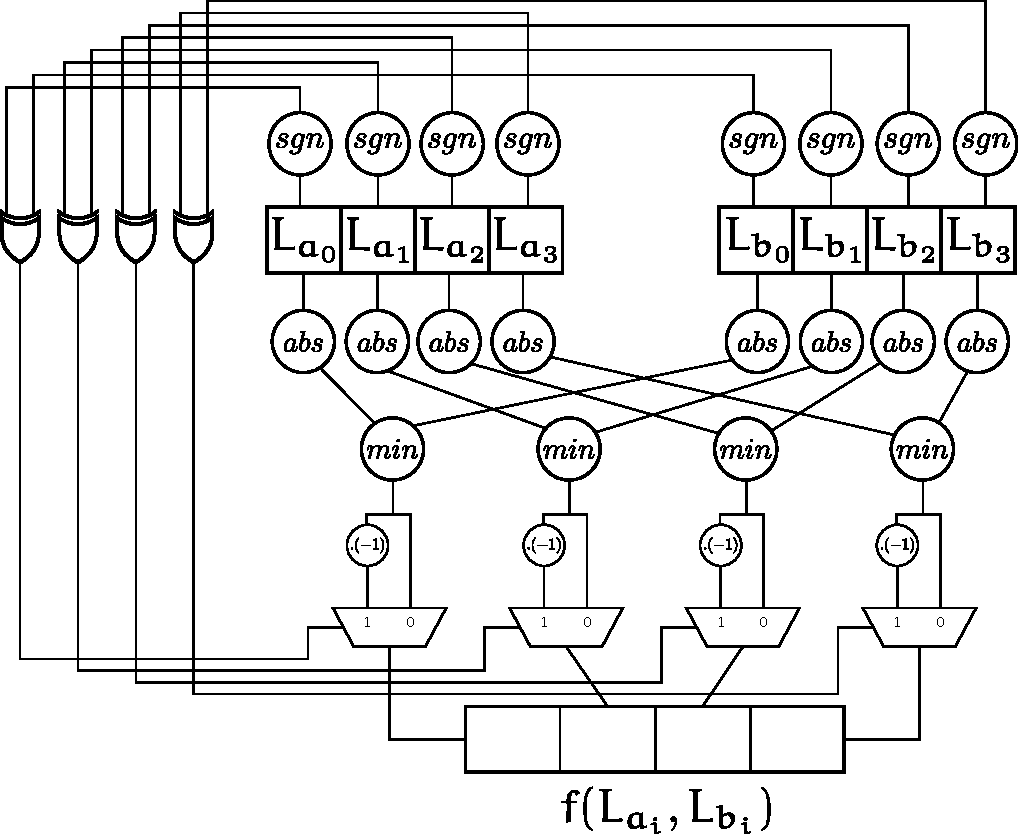
\includegraphics[scale=0.45]{main/ch3_fig/f_tie}
  \label{fig:f_tie}
  }
  \subfloat[Fonction $g$]{
  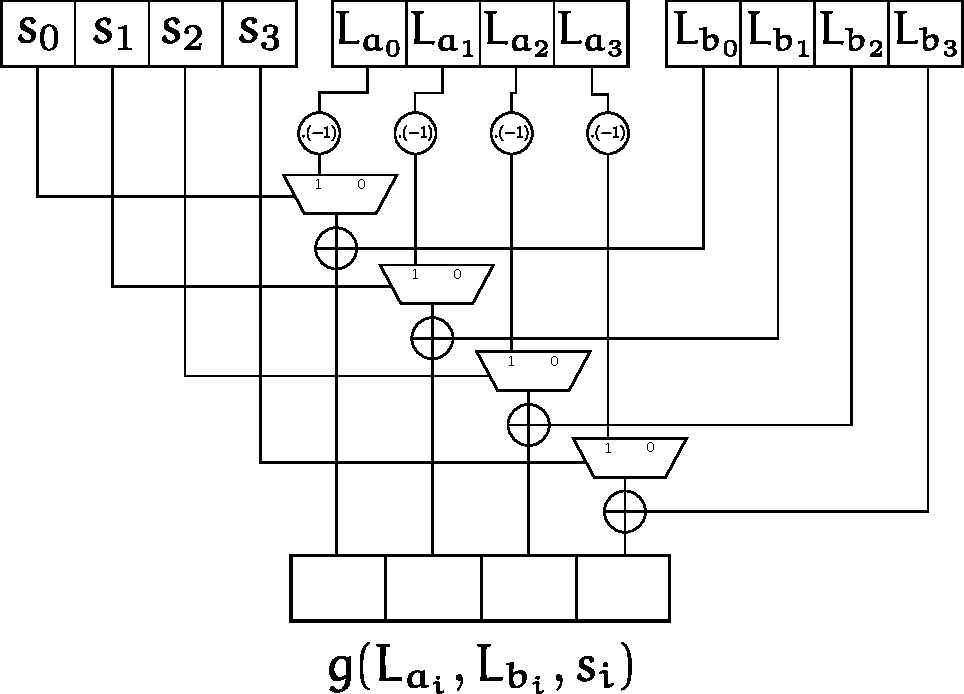
\includegraphics[scale=0.45]{main/ch3_fig/g_tie}
  \label{fig:g_tie}
  }
  \\\quad\quad\quad\quad\quad\quad
  \subfloat[Fonction \texttt{REP}]{
  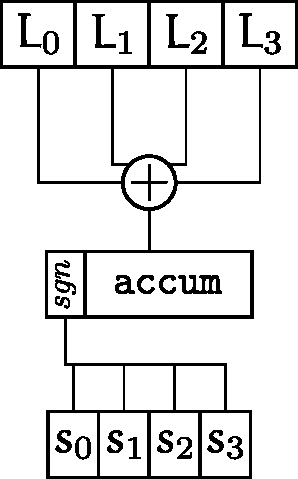
\includegraphics[scale=0.45]{main/ch3_fig/rep_tie}
  \label{fig:rep_tie}
  } \quad\quad\quad\quad\quad\quad\quad\quad\quad\quad
  \subfloat[Fonction \texttt{SPC}]{
  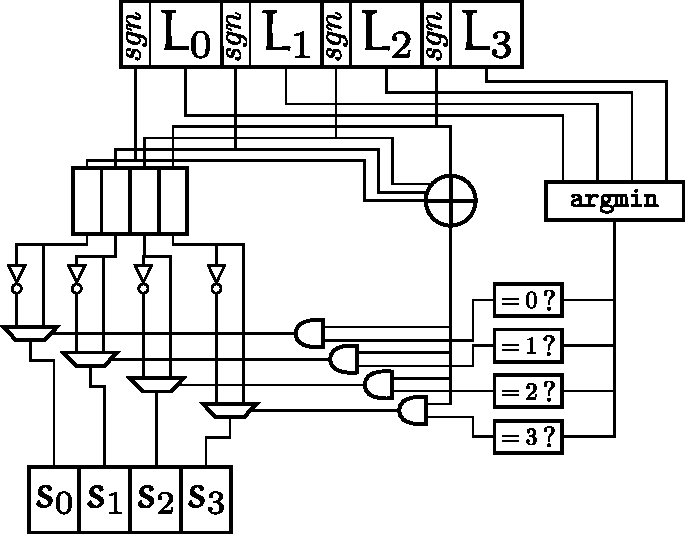
\includegraphics[scale=0.45]{main/ch3_fig/spc_tie}
  \label{fig:spc_tie}
  }
  \caption{Implémentations matérielles des instructions spécialisées.}
\end{figure}

Comme présenté dans la sous-section~\ref{subsec:pruning}, le traitement d'un \noeud de répétition consiste en l'addition de tous les LLRs d'entrée pour former la variable notée \og \texttt{accum} \fg dans la Figure~\ref{fig:rep_tie}. Puis de la détection du signe de cette variable, qui détermine le vecteur $s$ en sortie. Un arbre binaire est parcouru afin de réaliser l'addition nécessaire. Pour éviter tout débordement, la taille du registre de stockage de la variable \texttt{accum} est de 32 bits.

L'unité matérielle de traitement des \noeuds \texttt{SPC} est représentée dans la Figure~\ref{fig:spc_tie}. Il s'agit de l'unité la plus complexe à cause du tri nécessaire des LLRs. Aussi, le parallélisme de cet unité est limité à 8 dans notre implémentation.

\subsection{Instructions spécialisées \textit{simple-registre}}

Dans les implémentations logicielles classiques, la séquence d'opérations nécessaire à l'exécution des fonctions élémentaires polaires est la suivante : i) chargement depuis la mémoire cache vers les registres des variables d'entrée (LLRs et / ou sommes partielles), ii) calcul du résultat de la fonction élémentaire, en une ou plusieurs étapes, dont la sortie est stockée dans un registre, iii) sauvegarde de cette variable de sortie dans la mémoire cache du processeur.

\`A l'inverse, dans les implémentations matérielles présentées dans la sous-section \ref{subsec:hard_sc}, le chemin de données part de la sortie de la mémoire, passe par les fonctions combinatoires réalisant les fonctions polaires élémentaires, et finit à l'entrée de la mémoire. Ce chemin de données est parcouru en un seul cycle d'horloge. La méthode présentée dans cette sous-section, nommée \textit{simple-registre}, est conçue dans le but de reproduire le fonctionnement des implémentations matérielles de code polaire dans notre processeur.

\begin{figure}[t]
  \centering
  \subfloat[Unité matérielle \textit{simple-registre}.]{
  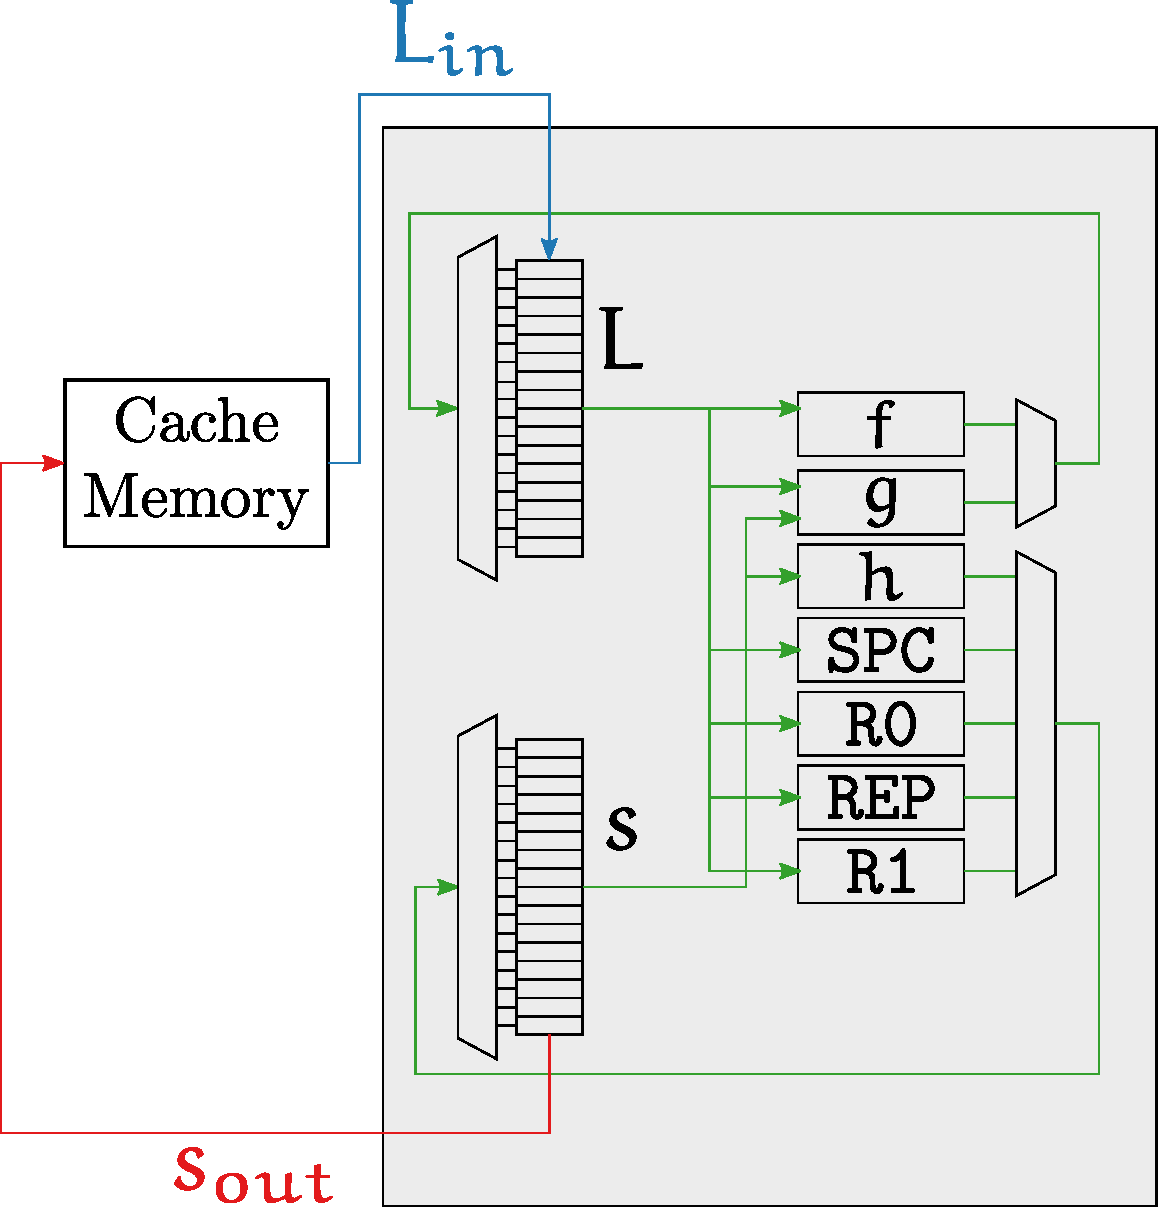
\includegraphics[scale=0.3]{main/ch3_fig/in_register_unit}
  \label{fig:in_register_unit}
  }\quad\quad\quad
  \subfloat[Un sous-arbre décodé grâce aux instructions \textit{simple-registre}.]{
  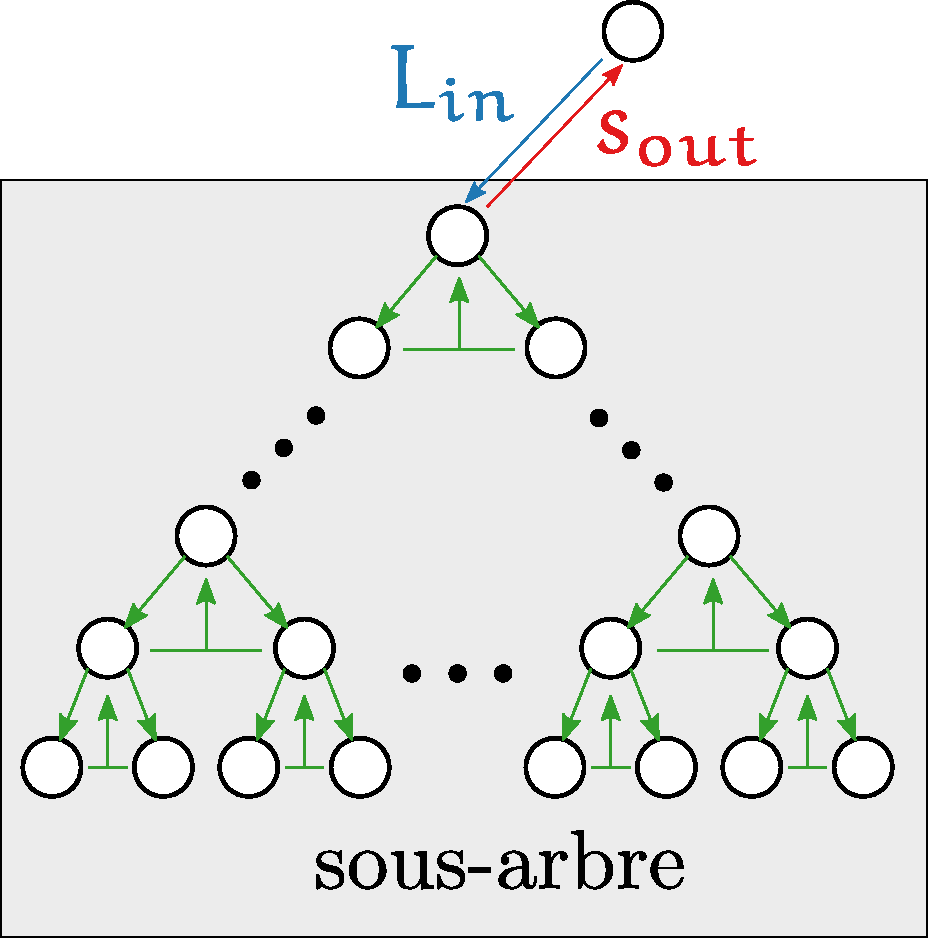
\includegraphics[scale=0.3]{main/ch3_fig/in_register_tree}
  \label{fig:in_register_tree}
  }
  \caption{Instructions \textit{simple-registre}.}
  \label{fig:simple-registre}
\end{figure}

La méthode \textit{simple-registre} est appliquée sur les sous-arbres de décodage dont le \noeud racine contient 64 LLRs. La Figure \ref{fig:in_register_tree} illustre un tel sous-arbre.
Ces 64 LLRs sont notés $\mathbold{L_{in}}$.
Lorsque le programme a généré les LLRs de la racine de ce sous-arbre, ceux-ci sont stockés dans un registre dédié.
Ce registre est noté $\mathbold{L}$ dans la Figure~\ref{fig:in_register_tree} qui représente l'unité matérielle qui réalise les instructions \textit{simple-registre}.
Le décodage du sous-arbre se fait ensuite intégralement à travers les registres, sans passer par la mémoire cache.
Les sommes partielles notées $\mathbold{s{out}}$ constituent la sortie de l'unité matérielle.
Cette méthode reproduit le fonctionnement des implémentations matérielles de l'algorithme SC : l'exécution d'une fonction élémentaire quelconque, comprenant la lecture et l'écriture de la donnée depuis le registre, est effectuée en un seul cycle d'horloge.

% \begin{figure}[htp]
% \centering
% 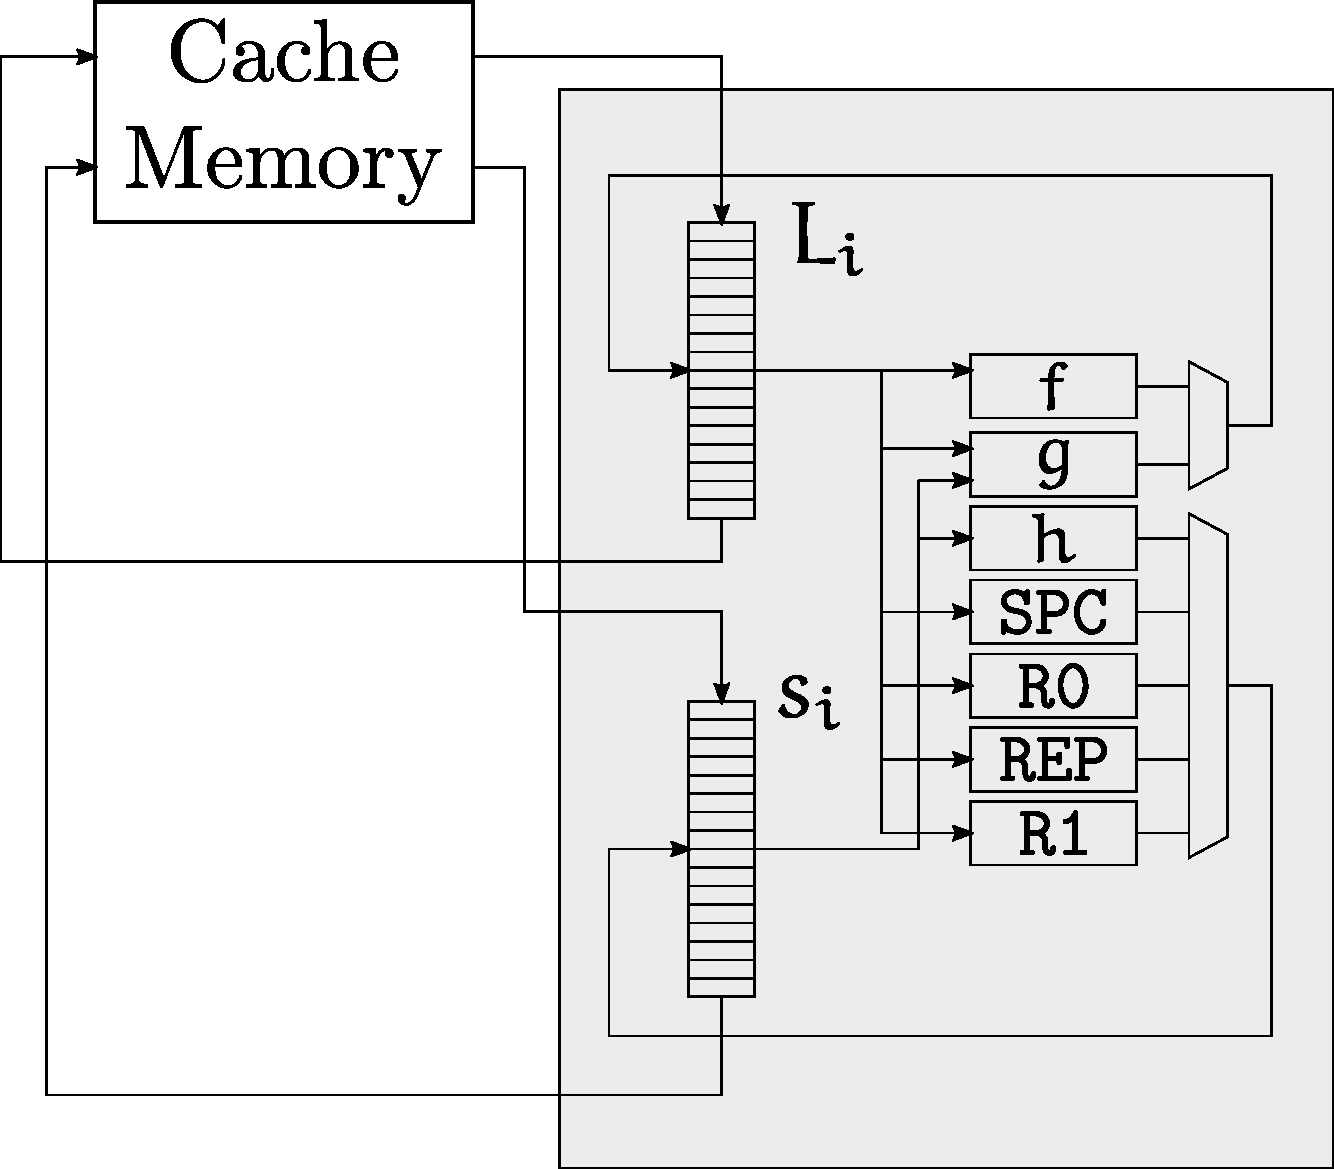
\includegraphics[width=0.7\textwidth]{main/ch3_fig/in_register}
% \caption{Instructions \textit{simple-registre}}
% \label{fig:simple-registre}
% \end{figure}




Elle résout également un problème récurrent des implémentations logicielles utilisant du parallélisme : l'alignement des données. En effet, pour pouvoir appliquer une fonction vectorielle des données de deux registres vectoriels, il est nécessaire de les aligner, ce qui nécessite d'effectuer des opérations supplémentaires. Dans l'implémentation \textit{simple-registre}, l'alignement est prévu en amont et implémenté dans l'unité matérielle. Aucune instruction supplémentaire n'est nécessaire. 

\subsection{Description logicielle}
L'ASIP ainsi proposé permet donc l'exécution efficace de l'algorithme de décodage de codes polaires SC. Le décodage est décrit de manière logicielle, en langage C augmenté des instructions spécialisées. Un extrait du code source est donné dans la Figure~\ref{fig:f_code}. Tout d'abord, les fichiers d'en-tête produits par les outils de conception définissent des types associés aux files de registres vectoriels (\texttt{VR512}). Afin de charger une donnée en mémoire cache vers ces registres vectoriels, il est nécessaire de créer des pointeurs vers ces variables de type (\texttt{VR512}). Les données sont ensuite chargées vers deux de ces registres vectoriels. La fonction spécialisée, ici la fonction \texttt{custom\_f\_64} est ensuite appliquée. Le résultat doit ensuite être stockée dans la mémoire cache.
\begin{figure}[hb]
\lstset{language=C++,
        basicstyle=\footnotesize\ttfamily,
        keywordstyle=\bfseries\color{green!40!black},
        commentstyle=\itshape\color{purple!40!black},
        identifierstyle=\color{blue},
        stringstyle=\color{orange},
        morecomment=[l][\color{magenta}]{\#}
}
\begin{lstlisting}[language=C++, numbers=left, numbersep=0.3em, tabsize=2, basicstyle=\footnotesize\ttfamily]
inline void f_64(signed char* la, 
                 signed char* lb, 
                 signed char* lc)
{
  p512_a = (VR512*) la; // transtyper de char* vers VR512
  p512_b = (VR512*) lb; // transtyper de char* vers VR512
  p512_c = (VR512*) lc; // transtyper de char* vers VR512

  v512_a = *p512_a; // chargement des donnees vers VR512
  v512_b = *p512_b; // chargement des donnees vers VR512
  
  // execution de l'instruction specialisee
  v512_c = custom_f_64(v512_a, v512_b); 
  
  // sauvegarde du resultat en cache
  *p512_c = v512_c;     
}
\end{lstlisting}
\caption{Description logicielle de l'exécution d'une instruction spécialisée.}
\label{fig:f_code}
\end{figure}

Lors du développement, il est apparu qu'il était difficile de réduire le temps passé à réaliser les opérations liées au parcours de l'arbre et aux différents tests. L'utilisation de l'option FLIX3 a permis de réduire ce temps, mais pas suffisamment. La technique de déroulage présentée en sous-section~\ref{subsec:unroll} permet de réduire ce temps. Dérouler le code améliore la performance au prix d'une flexibilité réduite. Il faut en effet générer une version différente du code pour un ensemble donné de paramètres.


\begin{figure}[htp]
\lstset{language=C++,
        basicstyle=\footnotesize\ttfamily,
        keywordstyle=\bfseries\color{green!40!black},
        commentstyle=\itshape\color{purple!40!black},
        identifierstyle=\color{blue},
        stringstyle=\color{orange},
        morecomment=[l][\color{magenta}]{\#}
}
\begin{lstlisting}[language=C++, numbers=left, numbersep=0.3em, tabsize=2, basicstyle=\footnotesize\ttfamily]
// fonction polaire spécialisée
void u_f_64(struct polar_operation& op)
{
    for(int i = 0; i < op.n_elmts; i+=64)
      F_64(op.arg0 + i, op.arg1 + i, op.arg2 + i);
}

// fonction polaire générique
typedef void (*polar_func)(struct polar_operation&);

// structure passée en argument de la fonction générique
struct polar_operation
{
  polar_func   p_func; // pointeur vers la fonction polaire spécialisée 

  signed char* arg0; // les arguments des fonctions polaires spécialisées
  signed char* arg1; // ces arguments sont souvent des adresses
  signed char* arg2;
  signed char* arg3;

  int          n_elmts; // le nombre d'éléments traités en parallèle
  int          off_s; // un offset nécessaire pour l'accès aux PSs
};

// le tableau polar_op_vec est initialisé lors de la construction
// du décodeur il contient la séquence des "polar operation"
std::vector<struct polar_operation> polar_op_vec;

// boucle principale du décodage
virtual void decode()
{
  const int n_op = polar_op_vec.size();
  for (int i = 0; i < n_op; i++)
  {
    // chaque fonction du tableau "polar_op_vec" est appelée
    polar_op_vec[i].p_func(polar_op_vec[i]); 
  }
}
\end{lstlisting}
\caption{Description logicielle du pseudo-déroulage.}
\label{fig:tensilica_code}
\end{figure}
Dans l'implémentation logicielle proposée, une alternative au déroulage, nommée pseudo-déroulage, est utilisée. Tout d'abord, toutes les fonctions élémentaires pour le décodage de code polaires possèdent le même prototype de fonctions dans la description logicielle. Le type de fonction à appliquer ($f$, $g$, $h$, \texttt{R0}, \texttt{R1}, \texttt{SPC}, \texttt{REP}) est passé en paramètre de la fonction, accompagné des adresses auxquelles accéder aux données à lire et écrire. De cette manière, il est possible de créer, un tableau contenant les pointeurs des fonctions à appeler. L'algorithme permettant de déterminer la séquence de fonctions à exécuter prend comme entrée le tableau de bits gelés correspondant au code polaire traité.

Comme ce tableau est généré par le processeur au moment de l'exécution, la généricité du décodeur est conservée. Les paramètres $N$ et $K$ ainsi que les indices de bits gelés sont données en entrée du programme et le processeur s'adapte automatiquement. Comme cela est détaillé dans la section suivante, ce pseudo-déroulage permet une réduction significatives du nombre de cycles d'horloges nécessaires au décodage d'un mot de code.


\section{Expérimentations et mesures}
\label{sec:tensilica_res}

\subsection{Mesure du gain lié à la spécialisation du processeur.}

Les codes polaires considérés ont été construits selon le document spécifiant les techniques de modulation et de codage pour le futur standard 5G \cite{3gpp_ts_2017-1}. 
La version académique des outils de design de Tensilica ne permettent pas d'effectuer une synthèse logique du processeur ou d'accéder à sa description RTL. Seules des estimations de la fréquence, de la consommation et de la surface occupée sont données. Nous avons sélectionné la technologie HPM 28nm de TSMC pour ces estimations.

Le Tableau \ref{tab:evolution_tensilica} présente l'impact des améliorations principales effectuées sur le processeur de base. Un code polaire (32768,29492) est décodé. Il s'agit là du code utilisé durant le développement du processeur. Les mémoires de données et d'instructions sont dimensionnées pour ce code. La première implémentation logicielle de l'algorithme SC sur l'architecture de base du processeur XTensa LX7 nécessite 7.3 millions de cycles pour décoder un mot de code. Nous voyons que l'architecture spécialisée pour le décodage de codes polaires combinée à la technique de pseudo-déroulage de la description logicielle permet de réduire le nombre de cycles d'un facteur 50. Les instructions \textit{multi-registres} sont responsables d'une grande partie de cette réduction. Elles permettent à elles seules de diminuer d'un ordre de grandeur le nombre de cycles nécessaire au décodage d'un mot de code.
 \begin{table}[htp]
    \renewcommand{\arraystretch}{1.1}
    \centering
    \caption{Impact de chaque amélioration de l'ASIP sur le nombre de cycles d'horloges nécessaires pour décoder une trame, le débit et la surface occupée. La taille des mémoires n'est pas prise en compte pour la surface occupée. Décodage d'un code polaire (32768,29492). Fréquence considérée : 835 MHz.}
    \label{tab:evolution_tensilica}
    {\small\resizebox{\linewidth}{!}{
    \begin{tabular}{l | c  c  c }
    \multirow{2}{*}{\textbf{Version du processeur}}       & \multirow{2}{*}{\textbf{\# cycles}}   & $\bm{\mathcal{T}_i}$  &   \textbf{Surface}          \\
                                                 &             &  \textbf{(Mb/s)}          &  \textbf{(portes)}          \\
    \cmidrule(lr){1-1}
    \cmidrule(lr){2-2}
    \cmidrule(lr){3-3}
    \cmidrule(lr){4-4}
Processeur de base                               &   $7.30\times10^6$  &   $3.4$            & $160000$             \\

+ instructions \textit{multi-registres} $f$,$g$ et $h$   &   $2.64\times10^6$  &   $9.3$            & $210500$             \\

+ instructions \textit{multi-registres} \texttt{R0},
\texttt{R1},\texttt{SPC} et \texttt{REP}         & $534.00\times10^3$  &   $ 46$            & $272000$             \\

+ FLIX3                                          & $296.00\times10^3$  &   $ 83$            & $311900$             \\

+ instructions \textit{simple-registre}              & $192.00\times10^3$  &   $128$            & $445500$             \\

+ pseudo unrolled                                & $151.00\times10^3$  &   $163$            & $445500$             \\
    \end{tabular}
    }}
  \end{table}


La puissance consommée estimée pour l'ASIP complet est de 111 mW, et la surface occupée est 0.475 mm\textsuperscript{2}. La fréquence estimée est 835 MHz. Cependant, les instructions spécialisées ne sont pas prises en compte pour l'estimation de la fréquence. En conséquence, un scénario plus réaliste où la fréquence de fonctionnement est 400 MHz est également présentée. Avec cette fréquence réduite, la consommation estimée devient 49 mW et la surface occupée 0.374 mm\textsuperscript{2}.

\subsection{Comparaison avec un processeur ARM}

Le logiciel AFF3CT développé par l'équipe CSN du laboratoire IMS de Bordeaux est utilisé pour exécuter une implémentation optimisée de l'algorithme SC sur un processeur ARM Cortex A57. La méthode de parallélisation \textit{intra-trame} est utilisée, et les LLRs sont représentés sur 8 bits avec virgule fixe. La taille des données gérées par les instructions NEON est de 128 bits, donc le parallélisme est égal à 16. Les résultats ici reportés ont été fournis par les auteurs de \cite{cassagne_energy_2016}. Dans ces résultats, la consommation de la mémoire RAM n'est pas prise en compte.
La Figure~\ref{fig:cycle_count} montre le nombre moyens de cycles d'horloges nécessaire à chaque processeur pour décoder une trame. Le processeur proposé réduit significativement le nombre de cycles grâce à l'utilisation d'unités matérielles de calcul spécialisées. La courbe tracée représente le rapport entre les nombres de cycle d'horloge de chaque processeur. Ce rapport est d'autant plus grand que $N$ est faible. Ceci est dû au fait que lorsque $N$ est faible, ce sont les instructions \textit{simple-registre} qui sont le plus utilisées. Or ces instructions sont les plus efficaces.
Cependant, ce nombre réduit de cycles d'horloge est contrebalancé par une fréquence réduite comme montré dans le Tableau~\ref{tab:asip}. Néanmoins, même dans le scénario le plus pessimiste, avec une fréquence de 400 MHz, le débit atteint par le processeur proposé est similaire à celui obtenu avec le processeur ARM. Qui plus est, l'énergie dépensée par bit décodé est 10 fois inférieur pour l'ASIP.
\begin{figure}[htp]
\centering
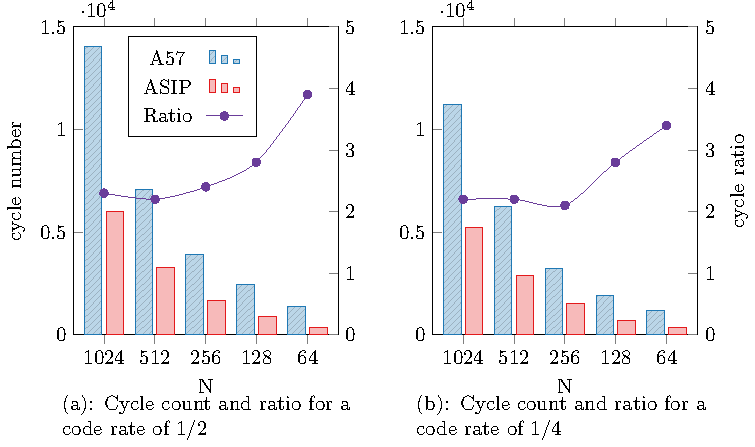
\includegraphics{main/ch3_fig/curves/cycle_count/cycle_count}
\caption{Comparaison du nombre de cycles de l'horloge nécessaires au décodage SC entre le Cortex ARM A57 et l'ASIP proposé.}
\label{fig:cycle_count}
\end{figure}

\subsection{Comparaison avec un processeur d'architecture x86}
Les débits, latences et l'énergie consommée par bit du décodeur logiciel SC inclus dans le logiciel AFF3CT ont également été mesurés sur un processeur Intel i7-4712HQ.
La puissance du \coeur est évaluée avec l'outil \texttt{powergadget} d'Intel. Seule la consommation du \coeur du processeur, excluant la consommation de la mémoire cache de niveau 3 et de la mémoire externe, est reportée. Cette fois-ci, le niveau de parallélisme est de 32 grâce à l'utilisation du jeu d'instructions AVX2. La fréquence du CPU mesurée durant l'exécution est de 3.3 GHz. Les résultats montrent que le débit et la latence des implémentations de décodeur SC sur les processeurs i7 sont bien meilleurs que ceux obtenus avec le processeur ASIP proposé ou avec le processeur ARM. Cependant, la consommation énergétique est moins bonne. Une implémentation \textit{inter-trame} permettrait d'augmenter cette efficacité énergétique, au prix d'une augmentation de la latence, comme démontré dans \cite{cassagne_energy_2016}.


\begin{table}[htp]
  \centering
  \caption{Comparaison de la latence, du débit et de la consommation énergétique de décodeurs SC sur différentes cibles matérielles.}
  \label{tab:asip}
%\scriptsize
  \begin{tabular}{ccccc}
    \toprule

    Target & $N$ & \begin{tabular}{c}Latency\\{[$\mu$s]}\end{tabular} & \begin{tabular}{c}Throughput\\{[Mb/s]}\end{tabular} & \begin{tabular}{c}$E_b$\\{[nJ]}\end{tabular} \\

    \cmidrule(lr){1-1}
    \cmidrule(lr){2-2}
    \cmidrule(lr){3-5}

    \multirow{4}{*}{\bf A57-1.1GHz}
     & $1024$  & $13$  & $38$  & $21$  \\
     & $512$   & $6.7$ & $38$  & $21$  \\
     & $256$   & $3.6$ & $35$  & $22$  \\
     & $128$   & $2.1$ & $30$  & $27$  \\
    \midrule
    \multirow{4}{*}{\bf i7-3.3GHz}
     & $1024$  & $2.3$ & $222$ & $47$  \\
     & $512$   & $1.4$ & $182$ & $57$  \\
     & $256$   & $0.8$ & $155$ & $68$  \\
     & $128$   & $0.5$ & $124$ & $85$  \\
    \midrule
    \multirow{4}{*}{\bf ASIP-835MHz}
     & $1024$  & $7.2$ & $71$  & $1.6$ \\
     & $512$   & $3.9$ & $66$  & $1.7$ \\
     & $256$   & $1.9$ & $65$  & $1.7$ \\
     & $128$   & $1.0$ & $62$  & $1.8$ \\
    \midrule
    \multirow{4}{*}{\bf ASIP-400MHz}
     & $1024$  & $15$ &  $34$  & $1.4$ \\
     & $512$   & $8.2$ & $31$  & $1.6$ \\
     & $256$   & $4.1$ & $31$  & $1.6$ \\
     & $128$   & $2.1$ & $30$  & $1.7$ \\
    \bottomrule
  \end{tabular}
\end{table}

\section*{Conclusion}

La première architecture de processeur ASIP spécialisée dans le décodage de codes polaires est présentée dans ce chapitre. Les outils logiciels de Tensilica permettent de spécialiser un processeur de type RISC. Après avoir détaillé la structure générales de ces microarchitectures RISC, nous expliquons comment elles peuvent être configurées et étendues par l'utilisation des outils logiciels de Tensilica. Les avantages et les enjeux liés à l'utilisation de tels outils de conception sont mis en avant.

Dans la seconde partie du chapitre, nous expliquons comment ces outils ont été mis en œuvre pour notre problématique : le décodage de codes polaires. Tout d'abord les paramètres de l'architecture RISC de base sont modifiés et adaptés. Entre autres, une fonctionnalité permettant le support d'un parallélisme d'instruction est activée, et la largeur du bus d'interface avec la mémoire de données est augmentée. Ensuite, des unités matérielles dédiées associées à des instructions spécialisées qui étendent le jeu d'instructions de base sont ajoutées. Enfin, une méthode de description logicielle nommée \og pseudo-déroulage \fg est proposé afin d'améliorer les performances de débit et de latence du processeur spécialisé conçu.

Dans une troisième partie, nous présentons et comparons le débit, la latence et la consommation du décodeur proposé avec les implémentations logicielles de codes polaires de l'état de l'art. Pour un code polaire (1024,512) décodé à l'aide de l'algorithme SC, le débit atteint est d'environ 70 Mb/s, dépassant les performances obtenues avec un processeur du marché de l'électronique embarquée. La consommation énergétique par rapport à ce même processeur est elle réduite d'un ordre de grandeur.

Bien que ces résultats soient prometteurs, plusieurs limites concernant l'utilisation des outils et de la méthodologie de conception des processeurs XTensa ont été identifiés. Tout d'abord, le défaut d'une licence complète empêche la génération du modèle matériel du processeur. Il est donc impossible de générer des résultats complets de synthèse et d'implémentation. Pour cette raison, les résultats obtenus sont des estimations fournies par l'outil, avec une marge d'erreur importante. Ensuite, le langage de descriptions matériel est le langage TIE, spécifique à la suite logicielle de Tensilica. Ceci limite les possibilités de réutilisation des unités matérielles conçues. D'autre part, une analyse attentive du code assembleur généré et des résultats de simulations montrent qu'une part très importante de la durée d'exécution est prise par les échanges de données entre la mémoire cache, les registres et les unités matérielles de calcul. La conception et l'ajout des instructions \textit{simple-registre} permettent de diminuer le nombre de ces échanges. Mais cette amélioration est partielle et ne peut pas être utilisée sur l'ensemble de l'arbre de décodage.

Plusieurs outils de conception d'ASIP ont été envisagés afin de résoudre ces problèmes. Parmi eux, la famille d'architectures \og TTA \fg a été sélectionnée pour créer le processeur présenté dans le chapitre suivant. Une des raisons de ce choix est la possibilité de contourner les registres et d'échanger les données directement entre la mémoire de données et les unités matérielles.